\section{Empirical Evaluation}
\label{Sec:evaluation}
To quantitatively assess the accuracy and efficiency of our
approach, we have conducted a case study following guidelines
from Runeson and H{\"o}st \cite{runeson2009guidelines}. In our evaluation, we address the
following research questions:

\begin{description}
\item [RQ1] How successful is \jsart in generating stable invariant assertions?
\item [RQ2] How effective is our overall regression testing approach in terms of correctly detecting faults?
% XXX perhaps it is better to discuss this in discussion section, not as a research question XXX \item [RQ3] What types of fault is the tool able to detect? What types of fault are not supported by the tool? 
\item [RQ3] What is the performance overhead of \jsart?
\end{description} 

The experimental data produced by \jsart is available for download.\footnoterecall{download}
%\curl{http://salt.ece.ubc.ca/content/jsart/}


\subsection{Experimental Objects}
Our study includes nine web-based systems in total. Six
are game applications, namely, SameGame, Tunnel, TicTacToe,
Symbol, ResizeMe, and GhostBusters.
Two of the web applications are Jason and Sofa, which are a personal and a company homepage, respectively. We further include TuduList, which is a web-based task management application. All these applications are open source and use \javascript on the client-side. 

\tabref{objectsChar_table} presents each application's ID, name, and resource, as well as the characteristics of the custom \javascript code, such as \javascript lines of code (LOC), number of functions, number of local and global variables, as well as the cyclomatic complexity (CC).
We use Eclipse IDE to count the \javascript lines of code, number of functions, number of local as well as global variables. JSmeter \curl{http://jsmeter.info} is used to compute the cyclomatic complexity.
We compute the cyclomatic complexity across all \javascript functions in the application.

% \begin{table}%[h!]
%\vspace{5pt}
        \caption{Objects of the case study.}
{\scriptsize
    \begin{center}
       
      %  \subtable[Experimental subjects and the corresponding exploration data]
            {
           \begin{tabular}{l|l|l} \hline
\thead{App ID} &  \thead{App Name} & \thead{Resource}  \\  \hline \hline

1 & SameGame  & \url{http://crawljax.com/same-game}  \\ \hline
           
2 & Tunnel  & \url{http://arcade.christianmontoya.com/tunnel/}  \\ \hline

3 & TicTacToe  &  \url{http://www.dynamicdrive.com/dynamicindex12/tictactoe.htm}  \\ \hline

4 & Symbol  & \url{http://10k.aneventapart.com/2/Uploads/652/}  \\ \hline

5 & ResizeMe & \url{http://10k.aneventapart.com/2/Uploads/594/}  \\ \hline

6 & GhostBusters  & \url{http://10k.aneventapart.com/2/Uploads/657/}   \\ \hline

7 & Jason  &  \url{http://jasonjulien.com/}   \\ \hline

8 & Sofa & \url{http://www.madebysofa.com/archive/}  \\ \hline

9 & TuduList  & \url{http://tudu.ess.ch/tudu/}  \\ \hline
\hline\end{tabular}\centering
            }
\label{Table:objects_table}
\end{center}
}  
\vspace{-0.1in} 
\end{table}



\begin{table*}[t]
\centering
%\vspace{5pt}
        \caption{Characteristics of the experimental objects.}
{\scriptsize
    \begin{center}
       
      %  \subtable[Experimental subjects and the corresponding exploration data]
            {
           % \hspace*{-0.4in}
           \begin{tabular}{c|l|c|c|c|c|c|l} \hline
\theadturn{App ID} &\theadturn{Name} &\theadturn{JS LOC} & \theadturn{\# Functions} & \theadturn{\# Local Vars} & \theadturn{\# Global Vars} &\theadturn{CC} &\thead{Resource}  \\  \hline \hline

1  & SameGame & 206 & 9 & 32 & 5 & 37 & \url{crawljax.com/same-game}   \\ \hline
           
2 & Tunnel & 334 & 32 & 18 & 13 & 39 & \url{arcade.christianmontoya.com/tunnel} \\ \hline

3 & TicTacToe & 239 & 11 & 22 & 23 & 83 &  \url{dynamicdrive.com/dynamicindex12/tictactoe.htm}  \\ \hline

4 & Symbol & 204 & 20 & 28 & 16 & 32 & \url{10k.aneventapart.com/2/Uploads/652}  \\ \hline

5 & ResizeMe & 45 & 5 & 4 & 7 & 2 & \url{10k.aneventapart.com/2/Uploads/594}   \\ \hline

6 & GhostBusters & 277 & 27 & 75 & 4 & 52 & \url{10k.aneventapart.com/2/Uploads/657}  \\ \hline

7 & Jason & 107 & 8 & 4 & 8 & 6 &  \url{jasonjulien.com}   \\ \hline

8 & Sofa & 102 & 22 & 2 & 1 & 5 & \url{madebysofa.com/archive}  \\ \hline

9 & TuduList & 2767 &  229 & 199 & 31 & 28  & \url{tudu.ess.ch/tudu}\\ \hline
\hline\end{tabular}\centering
            }
\label{Table:objectsChar_table}
\end{center}
}  
\vspace{-0.3in} 
\end{table*}

\subsection{Experimental Setup}
To run the experiment, we provide the URL of each experimental object to \jsart. In order
to produce representative execution traces, we navigate each application several times with different crawling settings. Crawling settings differ in the number of visited states, depth of crawling, crawling time, and clickable element types.
To obtain representative data traces, each of our experimental objects is navigated three times on average. Although \jsart can easily instrument the source code of imported \javascript libraries (e.g., jQuery, Prototype, etc), in our experiments we are merely 
interested in custom code written by developers, since we believe that is where most programming errors occur.

To evaluate our approach in terms of inferring stable invariant assertions (RQ1), we count the number of stable invariant assertions generated by \jsart
before and after performing the filtering step. As a last check, we execute the initial version of the application using the stable assertions to see whether
our filtered invariant assertions are reporting any false positives.

Once the stable invariant assertions are obtained for each web application, we perform regression testing on modified versions of each application (RQ2). To that end, in order to mimic regression faults, we produce twenty different versions for each web application by injecting twenty faults into the original version, one at a time. We categorize our faults according to the following fault model:

\begin{enumerate}
\item {\bf Modifying Conditional Statements}: This category is concerned with swapping consecutive conditional statements, changing the upper/lower bounds of
loop statements, as well as modifying the condition itself;  
\item {\bf Modifying Global/Local Variables}: In this category, global/local variables are changed by modifying their values at any point of the program, 
as well as removing or changing their names; 
\item {\bf Changing Function Parameters/Arguments}: This category is concerned with changing function parameters or function call arguments by swapping, removing, and renaming
parameters/arguments. Changing the sequence of consecutive function calls is also included in this category;   
\item {\bf DOM modifications}: Another type of fault, which is introduced in our fault model is modifying DOM properties at both \javascript code level and HTML code level.
\end{enumerate}

For each fault injection step, we randomly pick a \javascript function in the application code and seed a fault according to our fault model. We seed five faults from each category.
%However, if we are not able to inject upto 5 errors in a category, i.e. due to limited number of conditional statements or insufficient number of DOM invariants, 
%we increase the number of injected faults in the subsequent categories. 
%
%Thus the total number of faults is 20 per experimental object.

%We calculate the percentage of unstable invariants as follows:
%  $\frac{\mathit{\# UnstableInvariants}}{\mathit{\# UniqueInvariants}}\times100$

\begin{table}[t]
%\vspace{5pt}
        \caption{Properties of the invariant assertions generated by \jsart.}
{\scriptsize
    \begin{center}
       
      %  \subtable[Experimental subjects and the corresponding exploration data]
            {
           \begin{tabular}{c|c|c|c|c|c||c|c|c|c||c|c|c|c} \hline
\theadturn{App ID} & \theadturn{Trace Data (MB)} & \theadturn{\# Total Assertions} & \theadturn{\# Entry Assertions} & \theadturn{\# Exit Assertions} & \theadturn{\# DOM Assertions}
&\theadturn{\# Total Unstable Assertions} &\theadturn{\# Unstable Entry Assertions} &\theadturn{\# Unstable Exit Assertions} &\theadturn{\# Unstable DOM Assertions}
&\theadturn{\# Total Stable Assertions} &\theadturn{\# Stable Entry Assertions} &\theadturn{\# Stable Exit Assertions} &\theadturn{\# Stable DOM Assertions}\\  \hline \hline
%&\theadturn{\# Unique Invariants} 
1 & 8.6 & 303 & 120 & 171 & 12 & 0 & 0 & 0 & 0 & 303 & 120 & 171 & 12\\ \hline
           
2 & 124 & 2147 & 1048 & 1085 & 14 & 14 & 9 & 5 & 0 & 2133 & 1039 & 1080 & 14 \\ \hline

3  & 1.2  & 766 & 387 & 379 & 0 & 16 & 8 & 8 & 0 & 750 & 379 & 371 & 0\\ \hline

4 & 31.7 & 311 & 138 & 171 & 2 & 14 & 7 & 7 & 0 & 297 & 131 & 164 & 2\\ \hline

5  & 0.4 & 55 & 20 & 27 & 8 & 0 & 0 & 0 & 0 & 55 & 20 & 27 & 8\\ \hline

6  & 2.3 & 464 & 160 & 266 & 38 & 3 & 1 & 2 & 0 & 461 & 159 & 264 & 38 \\ \hline

7 & 1.2 & 29 & 4 & 6 & 19 & 0 & 0 & 0 & 0 & 29 & 4 & 6 & 19\\ \hline

8 & 0.1 & 20 & 2 & 2 & 16 & 0 & 0 & 0 & 0 & 20 & 2 & 2 & 16\\ \hline

9 & 2.6 & 163 & 58 & 104 & 1 & 0 & 0 & 0 & 0 & 163 & 58 & 104 & 1\\ \hline
\hline\end{tabular}\centering
            }
\label{Table:invariants_table}
\end{center}
}  
\vspace{-0.2in} 
\end{table}





To evaluate the effectiveness of \jsart (RQ2), we measure the precision and recall as follows:
\begin{description}
\item[Precision] is the rate of injected faults found by the tool that are correct: $\frac{\mathit{TP}}{\mathit{TP} + \mathit{FP}}$
\item[Recall] is the rate of correct injected faults that the tool finds: $\frac{\mathit{TP}}{\mathit{TP} + \mathit{FN}}$ 
\end{description}
where $TP$ (true positives), $FP$ (false positives), and $FN$ (false negatives) respectively represent the number of faults that are correctly detected, falsely reported, and missed.

To evaluate the performance of \jsart (RQ3), we measure the extra time needed to execute the application while assertion checks are in place. 


\subsection{Results}
In this section, we discuss the results of the case study with regard to our three research questions. 

\head{Generated Invariant Assertions.} \tabref{invariants_table} presents the data generated by our tool. For each web application, the table shows the total size of collected execution traces (MB), the total number of generated \javascript assertions, the number of assertions at entry point of the functions, the number
of assertions at exit point of the functions, and the number of DOM assertions. The unstable assertions before the filtering as well as the stable assertions after the filtering step are also presented. 
As shown in the table, for applications 1, 5, 7, 8, and 9, all the generated invariant assertions are stable and the filtering step does not remove any assertions. For the remaining four applications (2, 3, 4, 6), less than 5\% of the total invariant assertions are seen as unstable and removed in the filtering process. Thus, for all the experimental objects, the resulting stable assertions found by the tool is more than 95\% of the total assertions. Moreover, we do not observe any unstable DOM assertions. %This shows that most of the assertions found our tool are stable with only a few number of unstable assertions which are removed by the filtering step. 
In order to assure the stability of the resulting assertions, we examine the obtained assertions from the filtering step across multiple executions of the original application. The results show that all the resulting invariant assertions are truly stable since we do not observe any false positives.
%This also implies that our filtering mechanism successfully removes the small number of unstable assertions. 

\begin{table}[t]
%\vspace{5pt}
        \caption{Precision and Recall for \jsart fault detection.}
{\scriptsize
    \begin{center}
       
      %  \subtable[Experimental subjects and the corresponding exploration data]
            {
           \begin{tabular}{c|c|c|c|c|c} \hline
\thead{App ID} & \thead{\# FN} & \thead{\# FP} & \thead{\# TP} & \thead{Precision (\%)} & \thead{Recall (\%)}  \\  \hline \hline

1  & 2 & 0 & 18 & 100 & 90 \\ \hline
           
2 & 4 & 0 & 16 & 100  & 80 \\ \hline

3  & 1 & 0 & 19 & 100 & 95 \\ \hline

4 & 2 & 0 & 18 & 100 & 90 \\ \hline

5 & 0 & 0 & 20 & 100 & 100 \\ \hline

6 & 1 & 0 & 19 & 100 & 95  \\ \hline

7 & 0 & 0 & 20 & 100 & 100 \\ \hline

8 & 0 & 0 & 20 & 100 & 100 \\ \hline

9  & 1 & 0 & 19 & 100 & 95   \\ \hline
\hline\end{tabular}\centering
            }
\label{Table:precision_table}
\end{center}
}  
\vspace{-0.2in} 
\end{table}





As far as RQ1 is concerned, our findings indicate that (1) our tool is capable of automatically generating a high rate of \javascript invariant assertions, (2) the unstable assertions are less than 5\% of the total generated assertions, (3) the filtering technique is able to remove the few unstable assertions, and (4) all the remaining invariant assertions that \jsart outputs are stable, i.e., they do not produce any false positives on the same version of the web application.

%\ali{Three things should be made clear here: 1. Our tool is capable of generating JS assertions, 2. the filtering step removes the small number of unstable assertions, 3. the resulting stable assertions are truly stable.}
% our filtering mechanism is able to remove all detected unstable invariants.
% Thus, by executing the bug-free application using invaraints obtained from filtering step, we have not observed any unstable invaraints.
% our results imply that filtering mechansim is able to prevent from producing any potential reported false positives.
% Please note that for all experimental objects, unstable invariants are less than 10\% of the inferred unique invaraints. This shows that initial invariants generated by \jsart are fairly stable. 
% This implies that collected traces are converged to a set of stable invariants in a timely fashion.   
%\begin{table}%[h!]
%\vspace{5pt}
        \caption{Percentage of unstable invariants.}
{\scriptsize
    \begin{center}
       
      %  \subtable[Experimental subjects and the corresponding exploration data]
            {
           \begin{tabular}{p{1.1cm}|p{3.1cm}|p{3.1cm}} \hline
\thead{App ID} & \thead{Unstable Invariants BEFORE Filtering(\%)} & \thead{Unstable Invariants AFTER Filtering(\%)}  \\  \hline \hline

1  & 0 & 0  \\ \hline
           
2 & 4 & 0 \\ \hline

3 & 7 & 0\\ \hline

4 & 9  & 0\\ \hline

5  & 0  & 0 \\ \hline

6 &  1 & 0 \\ \hline

7  & 0  & 0\\ \hline

8 & 0  & 0\\ \hline

9 & 0  & 0    \\ \hline
\hline\end{tabular}\centering
            }
\label{Table:unstableInv_table}
\end{center}
}  
\vspace{-0.1in} 
\end{table}



\head{Effectiveness.} Since applications 3, 4, and 9 do not contain many DOM assertions, we were not able to inject 5 faults from the DOM modification category. Therefore, we randomly chose faults from the other fault model  categories.

In \tabref{precision_table}, we present the accuracy of \jsart in terms of its fault finding capability. 
The table shows the number of false negatives, false positives, true positives, as well as the percentages for precision and recall. As far as RQ2 is concerned, our results show that 
\jsart is very accurate in detecting faults. The precision is 100\%, meaning that all the injected faults, which are 
reported by the tool, are correct. This also implies that our filtering mechanism successfully eliminates unstable assertions as we do not observe any false positives. 
The recall oscillates between 80-100\%, which is caused by a low rate of  missed 
faults (discussed in \secref{discussion} under Limitations).
Therefore, as far as RQ2 is concerned, \jsart is able to successfully spot the injected faults with a  high accuracy rate.

\head{Performance.} \figref{overhead} depicts the total running time needed for executing each web application with and without 
the assertion code. Checking a fairly large number of assertions at runtime can be time consuming. Thus, to capture the effect of the added assertions on the execution time, we exploit a 2-scale diagram. As shown in \figref{overhead}, each experimental object is associated with two types of data. The left-hand Y-axis represents the running time (seconds), whereas the right-hand Y-axis shows the number of assertions.  This way we can observe how the number of assertions relates to the running time. As expected, the figure shows that by increasing the number of assertions, the running time increases to some degree. While the time overhead of around 20 seconds is more evident for the experimental object 2 (i.e., Tunnel with 2147 number of assertions), it is negligible for the rest of the experimental objects. Considering 
that Tunnel has 260 statements in total, the number of assertions instrumented in the code is eight times more than the number of statements in the 
original version. Therefore, it is reasonable to observe a small amount of overhead. Though assertions introduce some amount of overhead, 
it is worth mentioning that we have not experienced a noticeable change (i.e., freezing or slowed down execution) while running the application in the browser. 

Thus, as far as RQ3 is concerned, the amount of overhead introduced by our approach is 6 seconds on average for our experimental objects, which
is negligible during testing. %\ali{it's better to give an average number here: on average the overhead is x seconds, which is eligible during testing}
Furthermore, based on our observations, the assertions do not negatively affect the observable behaviour of the web applications in the browser.

\begin{figure}[t]
\centering
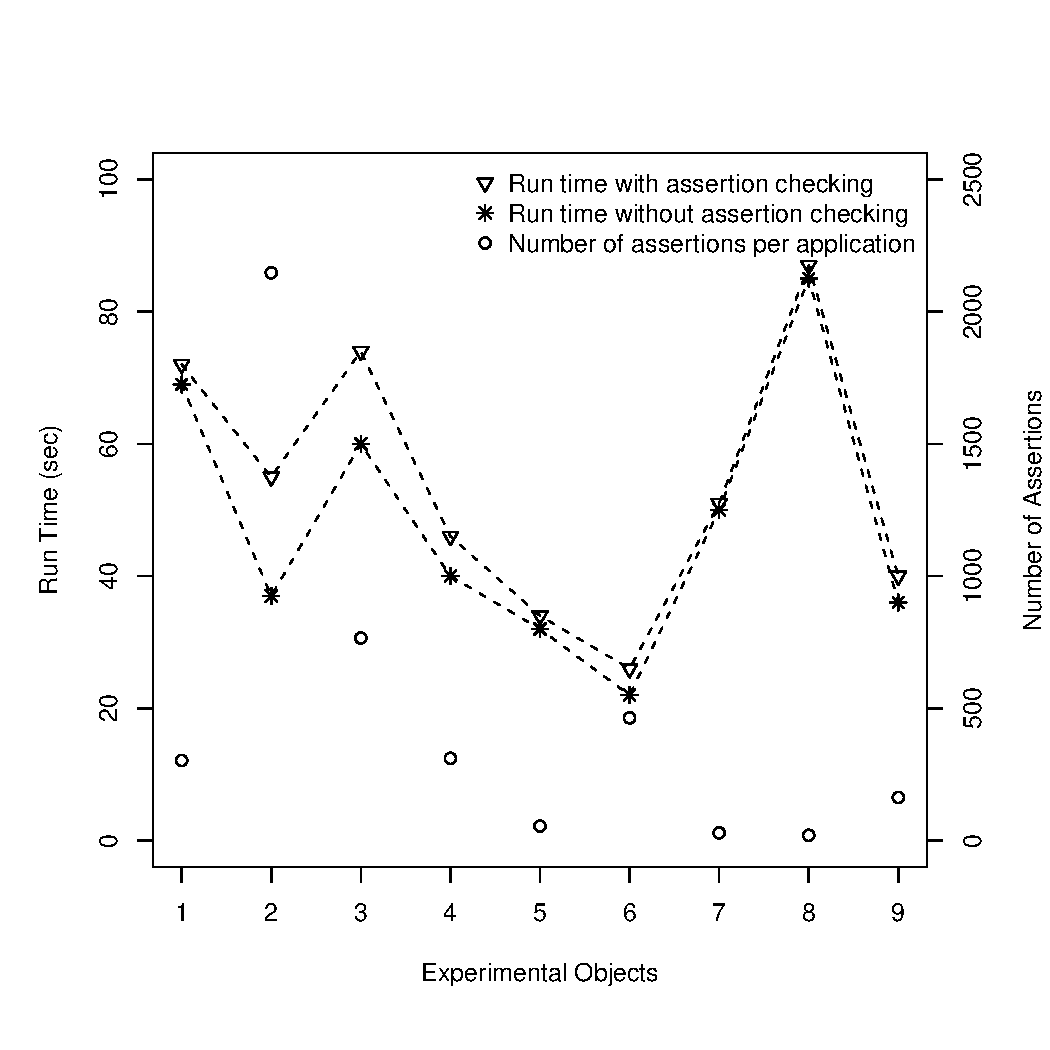
\includegraphics[width=0.68\hsize]{rscripts/overhead}
\mycaption{Performance plot of \jsart.}
\label{Fig:overhead}
%\vspace{-0.3in}
\end{figure}

  
  






